\clearpage

\section{Theorie}
\label{theorie}

%% Chipkarten %%
\subsection{Chipkarten}
\subsubsection{Entwicklung}
Wie bereits in der Einleitung erwähnt startete die Verbreitung der SIM-Karten
mit Einführung der Telefon- und Krankenversicherungs-Karten im Jahr 1985.
Bereits 6 Jahre später kamen die ersten Karten mit Mikroprozessoren - die \ac{SIM}-Karten
- zum Einsatz. Seit diesem Zeitpunkt haben sich die Chipkarten unter anderem
mit der enorm wachsenden Mobilfunkbranche stetig weiterentwickelt. Für diese
Arbeit ist vor allem die Chipkartenvariante \ac{SIM} wichtig.
Neben den klassischen Mikroprozessorkarten für \ac{GSM}-Netze wurden im Jahr
1998 damit begonnen JavaCards zu entwickeln. Diese verfügen über eine
Java-Laufzeitumgebung.

\subsubsection{Typen}
Bei Chipkarten wird zwischen zwei verschiedenen Typen unterschieden:
Speicher- und Prozessor-Karten \cite{chipkarten02}. Die Karten mit Mikroprozessoren
sind mittlerweile stärker vertreten als die reinen Speicherkarten.

Anwendungsgebiete für diese verschiedene Varianten von Chipkarten sind:
\begin{itemize}
\item Telekommunikation - \ac{SIM}-Karte
\item Bankwesen - elektronische Geldbörse
\item Gesundheitswesen - Krankenkassenkarte
\item Sicherheitskritische Anwendungen - Identifizierung und Authentifizierung
\item Service-Anwendungen - Pay-TV
\end{itemize}

\paragraph{Speicherkarten} werden dort verwendet wo kleine Datenmengen abrufbar
sein müssen. Meist wird dies in Form von \ac{EEPROM}-Speicherbausteinen realisiert,
die über ein serielles Protokoll beschrieben und gelesen werden können \cite{spitz11}.
Manche von ihnen sind dazu in der Lage über einfache Schaltungen simple Funktionen
zu integrieren. Nach Ausgabe ist es jedoch nicht mehr möglich die Funktionalitäten
zu ändern oder erweitern.

\paragraph{Prozessorkarten} erweitern die Speicherkarten um das Vorhandensein
eines Prozessors, der dazu in der Lage ist verschiedene (z.B. arithmetische)
Operationen auszuführen. Diese sind für rechenintensive Implementierungen
von Kryptoalgorithmen wie z.B. auch AES wichtig. Ebenfalls verfügt diese
Variante von Chipkarten über ein spezifisches Betriebssystem mithilfe derer
die verschiedenen Anwendungen ausgeführt werden können.
Neuere Architekturen erlauben es nach der Ausgabe der Karten Codestrecken
zu ändern oder erweitern.

\subsubsection{SIM-Karten}

\paragraph{Standardisierung}
\textit{SIM-Karten} folgen dem Standard der Chipkartentechnologie und sind in
ISO/IEC 786 definiert. Dort werden mechanische, physikalische und elektrische
Eigenschaften festgelegt.
So werden z.B. verschiedene Formfaktoren eingeführt, die Kompatibilität
auf mechanischer Ebene sicherstellt. Mobilfunkkarten müssen dem ID-000-Format
entsprechen, wohingegen Kreditkarten dem ID-1-Format entsprechen. Die physikalischen und elektrischen
Definitionen behandeln vor allem die Konformität der Kontaktflächen, damit
der Informationsaustausch zwischen Chipkarte und Lesegerät gesichert ist.
Eine Illustration befindet sich unter \Anhang{abb:pinbelegung_chipkarten}.

Neben den bereits genannten Aspekten wird auch das logische Verhalten des Betriebssystems
genau definiert. Interaktionen von Anwendungen mit dem Betriebssystem auf der Chipkarte
werden auf diesem Weg festgelegt. Desweiteren wird auch die Struktur des Dateisystems
genau beschrieben. Hier wird hohen Wert darauf gelegt auch auf kleine Datenmengen
granulare Rechtevergabe zu gewährleisten.
Eine Illustration befindet sich unter \Anhang{abb:filesystem_chipkarten}.

Benutzte Typen sind \ac{MF} für das Wurzelverzeichnis,
\ac{DF} für Dateien von Anwendungen sowie
\ac{EF} für die eigentlichen Dateien. Für jeden genannten Typ
existieren unterschiedliche Formate.

Grundlegend besteht eine Datei immer aus einem Header und einem Body. Während
der Body die Nutzdaten trägt, wird im Header der Dateityp und Zugriffsregeln
angegeben. Die Dateitypen beschreiben die genaue Struktur der Daten (zyklisch, linear fest,
linear flexibel,...).

\paragraph{Informationen} in Dateien auf SIM-Karten können entweder read-only- oder read-write-
Berechtigungen aufweisen. Je nach Art der Information. Sicherheits- und Identitätsbezogene
Dateien sind in der Regel read-only abgelegt, wobei SMS-Nachrichten sowie Kontaktdaten
read-write-fähig sein müssen. Unter anderem werden folgende Informationen auf der SIM-Karte gespeichert:

    \begin{tabularx}{\textwidth}{|l|X|}
    \hline
      \textbf{Name} & \textbf{Beschreibung} \\
    \hline
    \hline
      \ac{PIN} & Sicherheitscode zur Freischaltung der SIM-Karte \\
    \hline
    \hline
          \ac{PUK} & Sicherheitscode bei Wiederfreischaltung der SIM-Karte \\
    \hline
    \hline
      K\textsubscript{i} & Eindeutiger Authentisierungsschlüssel. Teilnehmer und Provider verfügen über ihn. \\
    \hline
    \hline
      \ac{IMSI} & Identifiziert einen Netzteilnehmer weltweit anhand dieser Zeichenfolge \\
    \hline
    \hline
      \ac{ICCID} & Identifiziert eine SIM-Karte weltweit anhand dieser Zahlenfolge (19-20 Stellen) \\
    \hline
    \hline
      \ac{LAI} & nimmt den aktuellen Locationcode beim eingewählten Punkt auf \\ 
    \hline
    \hline
      \ac{SMS} & Vom Teilnehmer empfangene oder versandte Nachrichten \\
    \hline
    \hline
      Kontakte & Vom Teilnehmer verwaltete Kontakte \\
    \hline
    \end{tabularx}

\paragraph{IMSI} Wie bereits aus der Tabelle hervorgeht identifiziert die \ac{IMSI} weltweit
einen Netzteilnehmer. Sie wird von Netzbetreibern ausgelesen und besteht aus drei Abschnitten:
\ac{MCC} (3 Stellen), \ac{MNC} (2-3 Stellen) und \ac{MSIN} ($\leq$ 10 Stellen).
Üblicherweise wird die \ac{IMSI} als 15-stellige Zahl angegeben, sofern das
Land keine andere Vorgabe macht. Nach dem \ac{MCC} werden in Europa beispielsweise 2-stellige \ac{MNC}s
verwendet. Nordamerika hingegen verwendet 3 Stellen. 

In Deutschlande wird der Code für z.B. die Telekom oder Vodafone wie folgt zusammengesetzt:

    \begin{tabularx}{\textwidth}{|l||l|l|X|}
    \hline
      \textbf{Betreiber} & \textbf{MCC} & \textbf{MNC} & \textbf{MSIN} \\
    \hline
    \hline
      Telekom & 262 & 01 & ... \\
    \hline
    \hline
      Vodafone & 262 & 02 & ...\\
    \hline
    \end{tabularx}%WIP

%% TODO #edit bei bedarf hier noch formfaktoren einbringen

\paragraph{Befehlsklassen} werden nach Dateiverwaltung, Authentisierung, Kryptographie
und Zählvariablen unterschieden\cite{spitz11}. Einzelne Kommandos, die in diese
Klassen eingeteilt sind, werden immer als \ac{APDU} versandt sowie empfangen.

Unter \Anhang{abb:befehlsklassen_chipkarten} befindet sich eine genauere
Auflistung der verschiedenen Befehle mit zugehörigen \ac{APDU}-Beispielen.

\paragraph{Sicherheit}
%% TODO EDIT
Über Chipkarten wird in \ac{GSM}- und \ac{UMTS}-Netzen Sicherheit abgebildet.
Sie fassen Kryptoalgorithmen auf Prozessoren sowie Kryptoschlüssel im
Filesystem. So werden beispielsweise die Kryptoalgorithmen A3, A5 und A8
auf SIM-Karten ausgeliefert, die zum Nachweis der Authentizität des Benutzers dienen.
Diese werden in Abschnitt \Verweis{authentifizierungsvorgang}
näher erläutert.

\paragraph{Angriffe} auf die Architektur waren vor allem vor den aktuell durch UMTS
integrierten Funktionen möglich. Hierzu gilt die Implementierung des \textit{COMP128}-Algorithmus.
Er ist dazu entwickelt dem A3- und A8-Algorithmus bei der GSM-Architektur zu realisieren.
Bei der Authentifikation des \ac{MS} beim \ac{AuC} erweist sich das eingesetzte Hashverfahren
als problematisch, da kleine Veränderungen in der Eingabe nicht ausreichend streuen. Somit
ist es möglich, dass auf der SIM-Karte gespeicherte geheime Schlüssel durch Kollisionsagriffe
ausgelesen werden können.

Ebenso ist es bedingt möglich SIM-Karten zu klonen. Mit zunehmender Anzahl von implementierten
Sicherheitsmechanismen steigt die Herausforderung an den Klonprozess. So reicht es mittlerweile
nicht mehr aus nur Informationen auszulesen und zu klnen.
Aufgrund der Tatsache, dass SIM-Karten mittlerweile nicht nur gespeicherte Informationen
ausliefern, sondern auch eigene Funktionen integrieren.
Dazu gehört beispielsweise das ableiten des Sitzungsschlüssels
mittels abgelegter und mit dem \ac{AuC} ausgetauschter Informationen. Ebenso wird das auslesen
von Informationen durch das bereits erwähnte Berechtigungssystem erschwert.

\paragraph{\ac{USIM}} ist die Weiterentwicklung der vorhergehenden normalen \ac{SIM}-Karte. Sie wird
im 3G- bzw. UMTS-Netz verwendet und erweitet das ursprüngliche Modell um einige Funktionen.
Diese Funktionen werden verwendet sofern das Gerät, in die sie eingesetzt wird den Standard
von USIM-Karten unterstützt. Manche Ausprägungen dieser Kartenvariante erlauben auch das Ablegen
von Mailadressen zu Kontakten. Der Hardwarekern dieser Architektur ist die \ac{UICC}.


\subsection{Mobilfunkstandards} % TODO: #edit umbenennen?
Technologien für den Mobilfunk basieren unter anderem auf den bereits beschriebenen
Chipkartenstandards. Weit verbreitete Standards für die Kommunikation sind
\textit{UMTS} und \textit{GSM}. Sie schließen neben den Chipkarten einen weiteren
Kontext mit ein. So gehören zu diesen Standards auch die Rollen des Mobiltelefons (\ac{MS}),
Authentifizierungsstellen (\ac{AuC}) sowie vielen weiteren Teilnehmern.

Die GSM- umd UMTS-Kryptoalgorithmen basieren auf symmetrischen Verfahren, die nicht
vollständig veröffentlicht wurden. Kryptoschlüssel müssen deshalb auf
Seiten der SIM-Karte und Authentifizierungsstelle parallel aufbewahrt werden.
Durch die Stelle der \ac{HLR} wird den \ac{AuC} die Verwaltung der Schlüssel erleichtert.
Der Anwender selbst meldet sich im \ac{BSS} bei GSM oder dem \ac{RNC} bei UMTS an \cite{spitz11},
die wiederum über das \ac{MSC} verbunden sind. Eine Illustration dieser Hierarchie
befindet sich unter \Anhang{abb:teilnehmer_telefonnetz}

\paragraph{GSM}
Möchte sich ein Teilnehmer im GSM-Mobilfunknetz anmelden, wird zuerst dessen Identität
gesichert in Form der \ac{TMSI} ausgehend von der SIM-Karte über das \ac{VLR} an das
\ac{HLR} übertragen. Aus der \ac{TMSI} und dem Standort, der sich aus dem \ac{VLR}
ergibt kann dann die \ac{IMSI} ermittelt werden \cite{spitz11}. In der
nachfolgenden Abbildung wird der Zusammenhang dargestellt.

\begin{figure}[htp]
 \begin{center}
  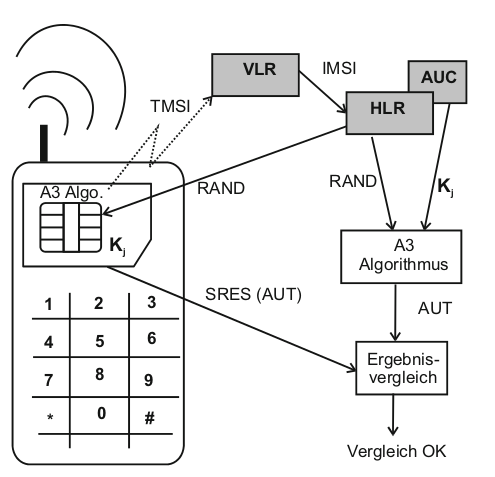
\includegraphics[width=180pt]{simauth_chipkartensicherheit}
 \end{center}
 \caption[Ablauf der GSM-Authentisierung]{Ablauf der GSM-Authentisierung \cite{spitz11}}
 \label{abb:simauth}
\end{figure}

Das \ac{HLR} überprüft dann mittels \ac{IMSI} die Benutzerrechte des Teilnehmers und
stößt den Authentifizierungsvorgang an. Selbiger wird dann auf Seite des
Mobilfunkteilnehmers sowie Providers ausgeführt und das Ergebnis verglichen.
Stimmen beide Ergebnisse überein werden weiterführend Sitzungsschlüssel erzeugt,
mit welchen die Nutzdaten (z.B. Sprache) sicher übertragen werden können.

\paragraph{UMTS} weist einige Unterschiede zum GSM-Mobilfunknetz auf, wobei die
vorhergehende Architektur aus Gründen der Abwärtskompatibilität weiterhin bestehen bleibt
(\ac{VLR},\ac{HLR},\ac{AuC}). Es wird die Variante der USIM als zentrale Chipkarte
eingesetzt. Der Ablauf der Authentisierung hingegen weicht vom Vorgänger etwas ab.
Dieser wird dadurch erweitert, dass das \ac{AuC} sich nun auch gegenüber der \ac{USIM}
authentisiert. Auf diesem wird die Sicherheit verbessert, da in beide Richtungen
geprüft wird, ob eine valide Gegenstelle vorliegt. \ac{IMSI}-Catchern wird es damit
schwerer gemacht eine Form des \textit{Man-In-The-Middle}-Angriffs zu ermöglichen.
Dementsprechend wird auch das Mitschneiden von Gesprächen erschwert. Weiterführend
wird im Gegensatz zu \ac{GSM} nun auch der Verkehr zwischen \ac{HLR} und \ac{VLR}
verschlüsselt realisiert \cite{spitz11}.
Die Authentisierung selbst über den Milenage-Algorithmus ist ebenfalls ausgebaut
und verfügt nun über weitere Vektoren, die im nachfolgenden Kapitel näher
erläutert werden.
%% TODO #edit hier vielleicht noch die abbildung für umts einfügen!?

%% Authentifizierungsvorgang %%
\subsection{Authentifizierungsvorgang}
\label{authentifizierungsvorgang}

Eine Darstellung des Authentifizierungsvorgangs ist in \Abbildung{kommunikationswege} zu
sehen. Diese beschreibt nur die Authentifizierung einer \ac{USIM}-Karte, aber nicht einer
GSM \ac{SIM}-Karte. \\
Die Authentifizierung ist recht umfangreich und soll hier anhand des Diagramms näher
erläutert werden. Anschließend wird auf die Stärken des Authentifizierungs\-
vorgangs eingegangen unter anderem in Bezug auf die Vorgehensweise in GSM.

 \subsubsection{Ablauf}
 
 \begin{figure}[htp]
 \begin{center}
  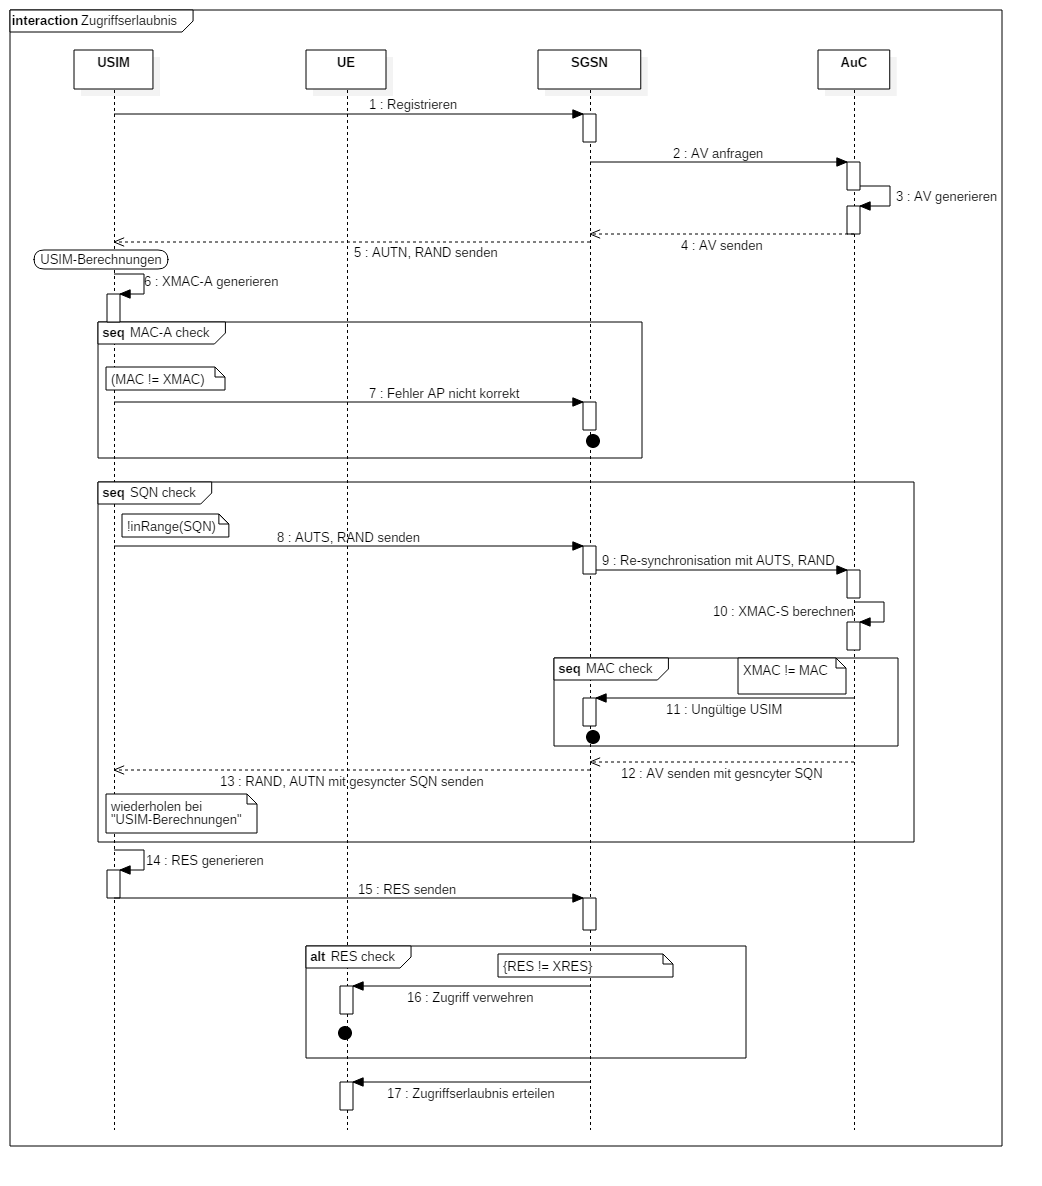
\includegraphics[width=440pt]{kommunikationswege}
 \end{center}
 \caption[Sequenzdiagramm über die Kommunikation zwischen SIM-Karte und Authentication Center]{Sequenzdiagramm über die Kommunikation}
 \label{fig:kommunikationswege}
\end{figure}

 Die Authentifizierung mit \ac{USIM}-Karten geschieht in zwei Richtungen. Es muss nicht nur die
 USIM verifizieren können, dass sie eine valide Karte ist, sondern der Netzprovider muss sich auch
 gegenüber der USIM verifizieren. Möchte eine USIM nun Zugang zum Netz erhalten schickt sie
 Registrierungsanfrage an den nächsten \ac{SGSN}. Diese fragt daraufhin beim \ac{AuC} des
 Netzproviders nach einem \ac{AV}. Dieser wird berechnet und nutzt dabei den in Kapitel
 \ref{milenage} auf S. \pageref{milenage} angesprochenen Milenage-Algorithmus. \\
 Der AV ist ein Quintett und besteht aus
 
 \begin{description}
  \item [RAND] Ein Zufallswert, der vom AuC jedes Mal neu generiert wird
  \item [XRES] Der Wert mit dem sich die USIM verifiziert
  \item [CK, IK] Für Verschlüsselungs- und Integritätsschutz bei der späteren Kommunikation
  \item [AUTN] Authentifizierungstoken, den die USIM benötigt. Ist selber ein Triplet aus:
  \begin{description}
   \item [SQN $\oplus$ AK] Eine Sequenznummer verschleiert durch einen Anonymitätsschlüssel
   \item [AMF] Providerspezifisches Managementfeld
   \item [MAC-A] Token zur Verifizierung des Netzwerks
  \end{description}
 \end{description}
 
 Die Werte XRES, CK und IK speichert der AP zwischen und RAND, sowie AUTN werden an die USIM
 weitergegeben als Antwort auf die Registrierungsanfrage.

 Mit Hilfe des RAND kann die USIM nun den XMAC-A berechnen, also den erwarteten Netzwerk\-
 token um zu überprüfen, dass die USIM sich bei dem richtigen Netzprovider registriert. Wenn XMAC-A
 und MAC-A nicht übereinstimmen, wird dem SGSN mitgeteilt, dass die Authentifizierung nicht erfolgreich
 war und die Kommunikation beendet.

 Sollten die Werte jedoch wie erwartet übereinstimmen, überprüft die USIM, ob die SQN im erlaubten
 Bereich ist. Wenn dem nicht so ist, bedeutet das nicht automatisch, dass die Kommunikation wieder
 beendet wird. Die USIM speichert die gültige SQN, was in Kapitel \Verweis{milenage-funktion}
 nochmal näher erläutert wird. Diese wird aktualisiert bei jeder Authentifizierungsanfrage und so kann
 es passieren, dass das AuC keine aktuelle SQN generiert hat und eine Resynchronisation vorgenommen
 werden muss, welche am Ende dieses Kapitels erklärt wird.
 
 Wenn die SQN im erlaubten Bereich liegt, generiert die USIM ihrerseits RES und schickt diesen an
 den SGSN. Der SGSN überprüft nun, ob XRES des Authenticaton Centers mit dem RES der USIM
 übereinstimmt. Je nach Ergebnis erteilt der SGSN dem \ac{UE} den Zutritt zum Mobilfunknetz oder
 nicht.
 
 \paragraph{Resynchronisation}
  Wie vorher in diesem Kapitel erwähnt kann es passieren, dass die SQN zwischen USIM und AuC
  nicht mehr synchron sind und deswegen resynchronisiert werden müssen. Dafür generiert die
  USIM ebenfalls einen RAND-Wert und einen AUTS-Token, welcher dem AUTN sehr ähnlich ist.
  Der AUTS hat im Gegensatz zum AUTN aber keinen AMF und statt dem MAC-A, wird ein MAC-S
  verschickt. Die SQN im AUTS, diel geschickt wird, ist die letzte gültige SQN, die die USIM erhalten
  hat. Aus dieser SQN kann das AuC nun eine gültige SQN berechnen. \\
  Ähnlich wie bei der Authentifizierung berechnet diesmal das AuC eine XMAC-S und vergleicht
  diese mit dem MAC-S aus dem AUTS. Sind diese nicht gleich geht wieder eine Meldung an den
  SGSN, die einen Fehler meldet und den Authentifizierungsvorgang beendet. Wenn diese Werte
  jedoch gleich sind, wird mit Hilfe der neuen SQN nochmal der AV berechnet und an den SGSN
  geschickt. Dieser gibt wieder AUTN und RAND an die USIM weiter welche die selben Schritte
  wie zuvor ausführt und diesmal zu dem Ergebnis kommen sollte, dass SQN im erlaubten
  Bereich liegt.
  
  Als Quelle für dieses Kapitel und für weitere Informationen dient \cite{3gpp.33.102}.
  
 \subsubsection{Stärken der UMTS Authentifizierung}
 Der Aufbau der \ac{UMTS}-Struktur beruht auf der selben Struktur, wie bereits \ac{GSM}.
 Denn auch wenn GSM einige Schwächen hat, zeigen die zehnjährige Existenz von GSM,
 dass die Sicherheitsarchitektur gut ist \cite{putz01}. Deshalb hat sich die \ac{3GPP} auch
 dazu entschieden, dass die Basis\-sicherheits\-features erhalten bleiben in UMTS. Konkret
 nennen Pütz, Schmitz und Martin (s. \cite{putz01}) unter anderem die folgenden Punkte:
 
 \begin{itemize}
  \item Vertraulichkeit der Teilnehmeridentität
  \item Teilnehmerauthentifizierung gegenüber dem Netzwerk
  \item Authentifizierung des Teilnehmers gegenüber der SIM
  \item Sicherheitsfunktionen ohne Aktion des Nutzers
  \item Eine Authentifizierungsmethode, die vom \ac{SN} durchgeführt wird, aber der gleichzeitig nur minimal vertraut werden muss
  \item Die Möglichkeit für jeden Provider eigene Authentifizierungsalgorithmen zu nutzen
 \end{itemize}
 
 Zusätzlich zu den Sicherheitsfeatures, die aus GSM übernommen wurden hat UMTS einige
 Schwächen aus GSM beseitigt oder zumindest das Ausnutzen eben jener erschwert. \\
 So können abgefangene \acp{AV} von Angreifern nicht wiederverwendet werden, da
 die SQN eingeführt wurde. \cite{putz01}\\
 Außerdem muss sich nun auch der Netzprovider der USIM gegenüber verifizieren, was
 Man-in-the-Middle Angriffe erschwert. \cite{putz01} \\
 Als letzter Punkt ist zu erwähnen, dass Daten noch länger verschlüsselt bleiben, als noch
 bei GSM, was die Angriffspunkte an denen man an die unverschlüsselten Daten direkt
 kommt weiter minimiert. \cite{spitz11}

%% Milenage Algorithmus %%
\subsection{Milenage Algorithmus}
\label{milenage}
Zwischen \ac{SIM}-Karte und Netzprovider muss eine sichere Authentifizierung und
Kommunikation gewährleistet werden können. Dies war, wie in Kapitel \Verweis{geschichte-usim}
bereits beschrieben, mit dem zuvor entwickelten Algorithmus des \ac{3GPP} nicht mehr
gewährleistet. Mit der Entwicklung des neuen Netzstandards wurde deshalb entschieden
auch einen neuen Algorithmus zu entwickeln, namentlich der Milenage Algorithmus. \\
Dieser verfügt über die sieben Funktionen \emph{f1}, \emph{f1*}, \emph{f2}, \emph{f3},
\emph{f4}, \emph{f5}, \emph{f5*} mit Hilfe derer eine sichere Authentifizierung und
Schlüsselgenerierung ermöglicht wird. Die Funktionen mit \emph{*} sind dabei lediglich für die
Re-synchonisation nötig. \\
3GPP hat, wie auch beim Vorgänger, diese Funktionen nicht näher spezifiziert und ermöglicht
den Netzprovidern eigene Lösungen zu implementieren. Deshalb wird nur beschrieben in
welchem Kontext diese Funktionen Anwendung finden und generelle Anforderungen
an diese Algorithmen definiert \cite{3gpp.35.205}.

Der Milenage Algorithmus hat wie erwähnt zwei Hauptaufgaben, nämlich einerseits die
Authentifizierung und anderereits die Generierung eines Schlüssel, um die versendeten Nachrichten zu
ver- und entschlüsseln.
% Wenn es um die Authentifizierung geht muss sich einerseits die USIM
% beziehungsweise das \ac{UE}, gegenüber dem Netzprovider authentifizieren, aber andererseits
% muss sich auch der Netzprovider gegenüber der USIM authentifizieren. Damit soll die
% Möglichkeit der Man-in-the-Middle Attacken reduziert werden, die es einem Außenstehenden
% erlauben die Kommunikation mitzulesen. Auch so genannte Replay-Attacken, bei denen zuvor
% aufgezeichnete Daten genutzt werden, sind nicht möglich, auf Grund der \acl{SQN} \cite{spitz11}.

In den nachfolgenden Unterkapiteln werden die Vorteile und die Funktionsweise des
Algorithmus, erläutert.

 \subsubsection{Warum Milenage sicher ist}
 In Kapitel \Verweis{authentifizierungsvorgang} wurde schon erklärt, dass das die Mechanismen
 zur Authentifizierung und zum Schlüsselaustausch angepasst wurden und durch einige
 Änderungen Vorteile mit sich bringen, aber auch der weiterentwickelte Algorithmus zur
 Berechnung der Daten weißt einige Vorteile auf. \\
 Ein wichtiger Punkt dabei ist, dass der Vorgänger geheim war, aber Milenage wurde öffentlich
 diskutiert. Der Vorteil der Offenlegung ist, dass auf diesem Weg Schwachstellen bemerkt werden
 bevor der Algorithmus implementiert ist. 
 
 Stephan Spitz zeigt in seinem Buch ``Kryptographie und IT-Sicherheit'' \cite{spitz11} drei
 wesentliche Gründe auf, die den Algorithmus sicher machen:
 
 \paragraph{Ergebnisse mit hoher Entropie}
 Wenn der Schlüssel \ac{K} unbekannt ist und die die Eingabeparameter \ac{SQN}, \ac{RAND}
 und \ac{AMF} variieren, dann werden ``sehr gute Pseudo-Zufalls-Ergebnisse mit einer hohen
 Entropie'' \cite{spitz11} erreicht. Dafür muss aber auch eine gute Blockchiffre wie AES
 eingesetzt werden.
 
 \paragraph{Keine Rückschlüsse auf K möglich}
 Wenn die Eingabe- und Ausgabeparameter der einzelnen Funktionen \emph{f1} bis \emph{f5}
 analysiert werden, lassen sich keine Rückschlüsse auf den Schlüssel K oder das \acf{OP}
 ziehen, auch nicht auf Teile dessen. Dies hängt unter anderem damit zusammen, dass K nicht
 direkt in die Funktionen eingeht.
 
 \paragraph{Schlüssellänge}
 Brut-Force-Angriffe, also stumpfes ausprobieren der Schlüssel, ist auf Grund der
 Schlüssellänge von 128 Bits dauert mit aktuellen Computern zu lange.
 
%% TODO #edit bei bedarf hier noch die Vorraussetzungen an die Parameter bzw. wie diese modifiziert werden können

 \subsubsection{Funktionsweise}
 \label{milenage-funktion}
 In Kapitel \Verweis{authentifizierungsvorgang} wurde beschrieben, welche Daten zwischen
 \ac{AuC} und \ac{UE} verschickt werden, jedoch nicht wie diese Daten generiert werden. Es
 gibt einige Werte, die auf der \ac{USIM} und der Datenbank des \ac{AuC} fest eingespeichert
 sind. Diese sind der \ac{OP} und \ac{K}, sowie jeweils fünf Rotations- und XOR-Konstanten
 (r1, ..., r5 und c1, ... c5). Welche Funktion welche Werte benötigt und generiert zeigt dabei \Abbildung{funktionsubersicht}.
 
 \begin{figure}[htp]
  \begin{center}
   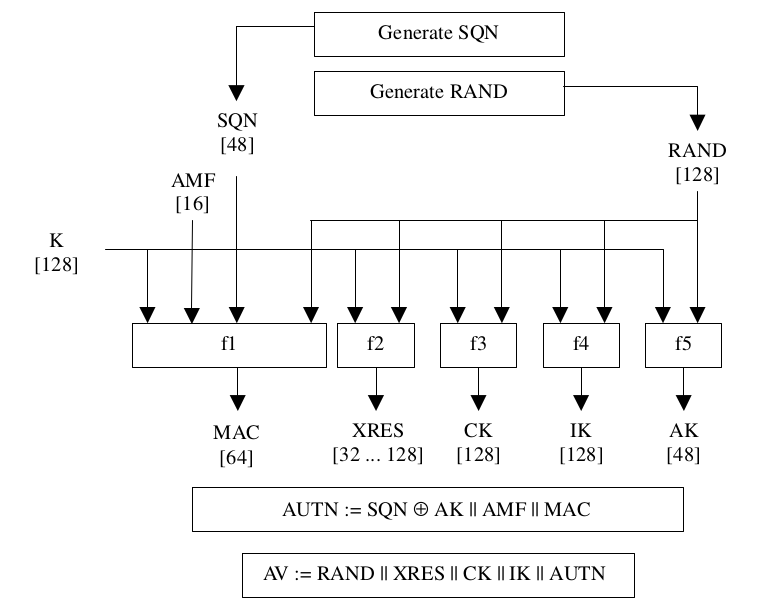
\includegraphics[width=300pt]{generation_of_authentication_vectors}
  \end{center}
  \caption[Übersicht über die Generierung der Authentifizierungsvektoren]{Übersicht über die Generierung der Authentifizierungsvektoren \cite{3gpp.33.102}}
  \label{fig:funktionsubersicht}
 \end{figure}
 
 In \Abbildung{funktionsubersicht} ist zu sehen, dass zu Beginn die \ac{SQN} generiert wird.
 Diese ist insgesamt 48 Bits lang und besteht aus den beiden Teilen SEQ und IND, mit SEQ als
 die eigentliche Sequenznummer und IND als Arrayindex. Dieser Index wird benötigt, da auf
 der SIM-Karte die letzten SQNs in einem Array gespeichert sind. Die empfohlene Arraygröße ist
 32, was für IND eine Länge von fünf Bits bedeutet. Mit diesem Index kann nachher die
 Aktualität der SEQ überprüft werden.\cite{3gpp.33.102} \\
 Für die Bildung der SEQ selbst gibt es drei verschiedene Möglichkeiten:
 \begin{itemize}
  \item teilweise zeitbasiert
  \item nicht zeitbasiert
  \item komplett zeitbasiert
 \end{itemize}
 
 Die einfachste Variante ist die nicht zeitbasierte Lösung, bei der lediglich ein Zähler hochgezählt
 wird mit jeder Authentifizierungsanfrage. Die SEQ ist initial also 0 und wird hochgezählt. Das
 \ac{AuC} speichert in einer Datenbank \cite{3gpp.33.102} zu jeder USIM die aktuelle SQN.
 Auf die anderen  Möglichkeiten wird hier nicht näher eingegangen, da sie in dieser Arbeit
 keine Anwendung fanden und deutlich komplexer sind.
 
 Als nächstes wird die \ac{RAND} gebildet. Das Verfahren, wie der Netzprovider diese RAND
 generiert darf nicht offen gelegt werden, da dies die Sicherheit stark beeinflussen würde. Die
 Spezifikation gibt deshalb für die Generierung der RAND keine Empfehlung, wie für die anderen
 Werte. Generell handelt es sich bei der RAND um eine 128-bit lange Zufallszahl, die für alle
 anderen Funktion benötigt wird.
 
 \Abbildung{funktionsubersicht} zeigt zwar, welche Variablen in die Funktionen einfließen und
 welche Werte sie zurückgeben, aber sie zeigt nicht näher wie diese Werte nun in den einzelnen
 Funktionen angewendet werden. Dies zeigt \Abbildung{schematisch_milenage} besser. Dort ist
 zu erkennen, dass \emph{f2} bis \emph{f5*} nach dem selben Schema berechnet werden können und
 \emph{f1}, sowie \emph{f1*} noch einige zusätzliche Parameter benötigen.
 
 Zunächst die Erklärung der Symbole sowie einiger weiterer Abkürzungen. OPc wird durch
 folgende Formel generiert:
 \begin{center}
  $OP_{C} = OP \oplus E(OP)_{K}$
 \end{center}
 
 $E()$ ist die Blockchiffre. In diesem Falle wird also \ac{OP} mit dem Schlüssel \ac{K}
 verschlüsselt. Welche Verschlüsselung gewählt wird, wird von 3GPP nicht vorgegeben. In
 dieser Arbeit wurde \ac{AES} verwendet, welche im Kapitel \Verweis{aes} näher beschrieben wird. \\
 Der verschlüsselte OP wird dann im zweiten Schritt über XOR ($\oplus$) mit dem ursprünglichen
 OP verknüpft.
 
 \begin{figure}[ht]
  \begin{center}
   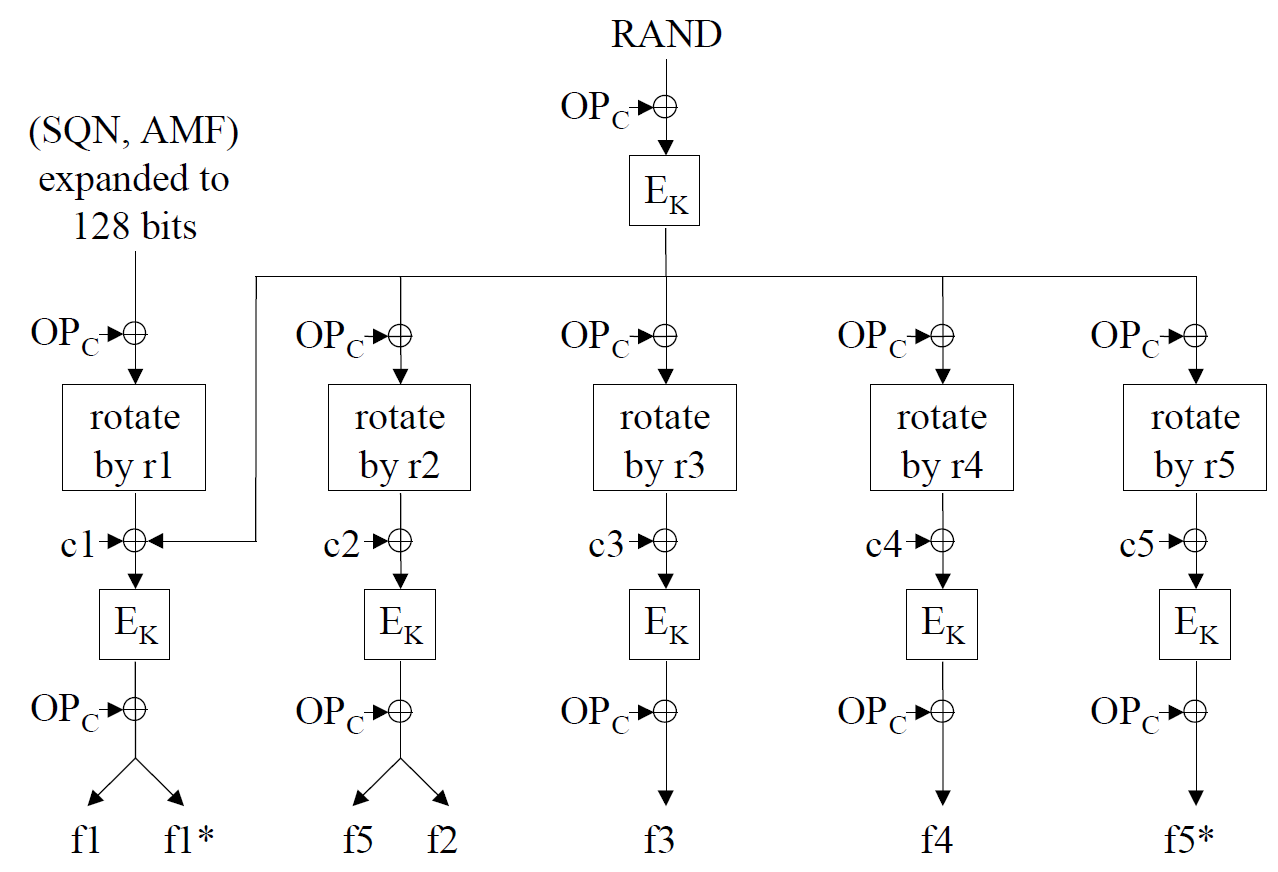
\includegraphics[width=400pt]{detailed_generation_of_authentication_vectors}
  \end{center}
  \caption[Schematische Darstellung der Berechnung der Authentifizierungsvektoren]{Schematische Darstellung der Berechnung \cite{3gpp.33.102}}
  \label{fig:schematisch_milenage}
 \end{figure}
 
 In \Abbildung{schematisch_milenage} ist weiterhin der Funktionsblock ``rotate by r'' zu lesen.
 Beim rotieren wird der Eingabewert um die Anzahl an Bits des Wertes von r rechts rotiert und
 die Bits die herausfallen links wieder eingefügt. Beispielsweise wird aus 110101 bei einem
 Rotationswert r von 2: 011101.
 
 Mit den genannten Infos ist verständlich, dass die Funktionen \emph{f2} bis \emph{f5*}
 ausgehen von einem verschlüsselten $RAND \oplus OP_C$, welcher in der Dokumentation
 auch als TEMP bezeichnet wird. Dieser Wert wieder wieder über XOR-mit $OP_ C$ verknüpft
 und um die entsprechende Rotationskonstante r rotiert. Im Anschluss wieder eine XOR
 Verknüpfung mit der speziellen XOR-Konstante c und die Chiffrierung des Ausgabewertes. Im
 letzten Schritt wird dieser dann nochmal über XOR mit $OP_{C}$ verknüpft. \\
 Wie die \Abbildung{schematisch_milenage} zeigt funktionieren \emph{f1} und {f1*} sehr
 ähnlich. Bevor jedoch TEMP in die Berechnung einfließt wird SQN und AMF auf 128 Bits
 erweitert und bekommt in der Dokumentation die Bezeichnung IN1. IN1 besteht aus SQN und
 AMF abwechselnd konkateniert, also SQN $\|$ AMF $\|$ SQN $\|$ AMF. \cite{3gpp.33.102}
 
%% AES/Rijndael %%
\subsection{AES / Rijndael}
\label{aes}
 Rijndael oder \ac{AES} sind beide Blockverschlüsselungen. Das bedeutet, dass der zu
 verschlüsselnde Text in gleich große Blöcke aufgeteilt wird und jeder Block mit einem Schlüssel
 chiffriert wird. Die Blocklänge des verschlüsselten Text bleibt dabei gleich. \\
 Der Unterschied zwischen Rijndael und AES besteht lediglich in der Länge der Text- uns
 Schlüsselblöcke und ist sonst identisch. Für Rijndael gilt, dass Block- und Schlüssellänge
 unabhängig von einander auf Vielfache von 32 Bits definiert werden können. Minimal müssen
 beide aber 128 Bits lang sein und maximal 256 Bits \cite{daemon02}. \\
 AES auf der anderen Seite hat die Blocklänge auf 128 Bits festgelegt und die Schlüssel\-länge
 darf nur 128, 192 oder 256 Bits betragen \cite{AES-FIPS}.
 
 Im folgenden soll kurz die Geschichte von AES beziehungsweise Rijndael erläutert werden und
 wie der Verschlüsselungs\-algorithmus der beiden funktioniert. Nicht angesprochen wird der
 Entschlüsselungs\-algorithmus, da der für diese Arbeit keine Relevanz hat.
 
 \subsubsection{Geschichte}
 \label{aes-geschichte}
 Die erste Blockverschlüsselung, die vom \ac{NIST} 1977 offiziell übernommen wurde, war
 \ac{DES} und basierte auf einer überarbeiteten Version der Blockverschlüsselung Lucifer. Bei
 DES betrug die Blockgröße nur 64 Bits, was lange Zeit ausreichend war, aber mit Fortschreiten
 der Rechenleistungen nicht mehr lange genügen würde gegen Brute-Force Angriffen (weitere
 Argumente finden sich in \cite{paar10}. Es gab deswegen die Empfehlung den dreifach DES zu
 nutzen, aber der war nochmal langsamer, als der einfache DES, weshalb das NIST eine neue
 Blockverschlüsselung suchte über eine Ausschreibung (1997).
 
 An die neue Verschlüsselung wurden folgende Bedingungen gestellt:
\begin{itemize}
 \item Blockverschlüsselung mit einer Blocklänge von 128 Bits
 \item Die drei Schlüssellängen 128. 192 und 256 Bits müssen unterstützt werden
 \item Sicherheitslevel ähnlich anderer Algorithmen
 \item Effizient in Soft- und Hardware
\end{itemize} 

Die Suche nach dem neuen Algorithmus fand öffentlich statt, sodass sich jeder auf der ganzen
Welt beteiligen konnte und im August 1999 fünf Finalisten gekürt wurden. Dabei wurden
öffentlich die Vor- und Nachteile der einzelnen Algorithmen diskutiert und Ende 2000 hat NIST
mit Rijndael den Gewinner bekannt gegeben. Dieser wurde von den beiden Belgiern Joan
Daemon und Vincent Rijmen entwickelt.

An dieser Stelle sei auch zu erwähnen, dass die \ac{NSA} sehr viel vertrauen in AES hat. So hat
diese die generelle Erlaubnis erteilt als \emph{SECRET} eingestufte Dokumente mit AES zu
verschlüsseln und selbst als \emph{TOP SECRET} eingestufte Dokumente dürfen mit einer
Schlüssellänge von 192 oder 256Bits verschlüsselt werden. \cite{paar10}
 
 \subsubsection{Funktionsweise}
 \label{aes-funktion}
 Bei der Blockverschlüsselung gibt es fünf verschiedene Betriebsmodi, die in der ISO/IEC 10116:2006
 \cite{ISO10116} beschrieben sind. Diese Betriebsmodi beschreiben wie ein Text bestehend aus
 mehreren Blöcken verschlüsselt wird.
 
  \paragraph{Electronic Codeblock (ECB)}
   Jeder Textblock wird unabhängig vom vorherigen Block verschlüsselt. Daraus resultieren vor allem
   zwei Dinge. Zum einen bewirkt eine Vertauschung der Blöcke im chiffrierten Text zur gleichen Vertauschung
   im entschlüsselten Text und zum anderen beeinflusst ein Fehler bei der Entschlüsselung eines Blocks
   nicht die anderen Blöcke. Es wird deshalb davon abgeraten diesen Modus zu verwenden bei mehr
   als einem Block.

  \paragraph{Cipher Block Chaining (CBC)}
   Beim CBC werden die Schwächen von ECB verkleinert, in dem eine Verkettung der Blöcke vorgenommen
   wird. So gibt es beim ersten Block zusätzlich zum Schlüssel noch einen Initialisierungsvektor. Bei den
   folgenden Textblöcken wird der Schlüssel mit dem vorhergehenden verschlüsselten Textblock
   verknüpft. Dadurch können Blöcke nicht mehr vertauscht werden und wenn ein Fehler bei der Ent\-
   schlüsselung in einem Block passiert ist zusätzlich zu diesem auch der nachfolgende Block nicht mehr
   zu entschlüsseln.
   
  Neben den beiden genannten Modi existieren noch ``Cipher Feedback'', ``Output Feedback'' und
  ``Counter''. Auf diese soll hier aber nicht näher eingegangen werden, da diese Elemente der
  Stromchiffre nutzen. Ihre Erklärung wäre deshalb für diesen Rahmen zu umfangreich, da beim
  Mileange-Algorithmus nur keine Zeichenketten länger oder kürzer als ein Block verschlüsselt
  werden. Das ist auch der Grund warum bei Milenage bedenkenlos der ECB eingesetzt werden kann.
  
  Beim AES-Algorithmus werden nicht nur Teile sondern immer alle 128 Bits bearbeitet, weshalb die
  Anzahl der Iterationen relativ gering ist und den Algorithmus schnell macht. Bei einer Schlüssellänge
  von 128 Bits werden 10 Runden benötigt, bei 192 Bits 12 und bei der Schlüssellänge von 256 Bits
  sind 14 Runden nötig. In jeder Runde werden vier Funktionen auf den Textblock angewendet, um
  den Textblock gut zu verschlüsseln.
  
  Damit der Textblock mit dem Schlüssel verschlüsselt werden können, müssen beide in ein rechteckiges
  Array aus Bytes transformiert werden. Die Anzahl der Reihen ist immer vier, aber die Anzahl der Spalten
  variiert je nach Textlänge. Mit der Umwandlung des Textblocks in das Array, spricht man vom Zustand
  und der umgewandelte Schlüssel ist nun der Chiffrierschlüssel. \\
  Der Zustand ist bei AES immer vier Spalten breit und der Chiffrierschlüssel vier, sechs oder acht Spalten
  breit. In beiden Fällen wird das Array zeilenweise gebildet. Das bedeutet das bei einer Blocklänge von
  128 Bits in den ersten vier Arrayelementen des Zustands die ersten 32 Bits des Blocks stehen.
  
  Nachfolgend werden nun die vier Funktionen beschrieben die den Zustand verändern.
  
  \paragraph{SubBytes}
   Bei der SubBytes-Transformation handelt es sich um eine nicht-lineare Bytesubstitution, welche
   separat auf jedes Byte des Status angewendet wird. Die Substitutionstabelle, auch S-Box genannt,
   ist 16 x 16 Felder groß und ist damit eine bijektive Abbildung aller 256 möglichen Eingabemöglichkeiten.
   Wie die Tabelle gebildet wird, wird an dieser Stelle nicht näher beschrieben, aber im \Anhang{abb:s-box}
   befindet sich die Tabelle.
   
   Mit dem Wert das Statuselements wird nun der Wert aus der Substitutionstabelle ermittelt. Die ersten vier
   Bits geben die Zeile vor und die letzten viert Bits die Spalte. So wird beispielsweise der Wert $8D_{16}$ mit
   $5D_{16}$ substituiert.
   
  \paragraph{ShiftRows}
   Bei dieser Funktion werden die Bytes in jeder Zeile des Zustands-Arrays zirkulär verschoben. Das bedeutet,
   dass die einzelnen Bytes vorne, also links, ``rausgeschoben'' werden und hinten/rechts, wieder
   ``reingeschoben''. Dabei ist  die Anzahl der Verschiebungen in jeder Zeile unterschiedlich. In Zeile eins wird
   gar nicht verschoben, in Zeile zwei um ein Byte, Zeile drei um zwei Bytes und in Zeile vier das Array um drei
   Bytes verschoben.
   
   In einer vierten Zeile würde somit aus dem String $3B | 2A | 34 | 71$ der String $71 | 3B | 2A | 34$ werden.
   
  \paragraph{MixColumns}
   In der MixColumns-Transformation wird nicht jedes Byte einzeln transformiert, sonder die gesamte Spalte.
   Die Berechnung ist hierbei etwas umfangreicher, als in den Transformationen zuvor. Nehmen wir eine Spalte
   $j$, dann wird folgende Berechnung durchgeführt:
   
    \begin{equation*}
     \begin{split}
     b_{0,j} = T_2(a_{0,j}) \oplus T_3(a_{1,j}) \oplus a_{2,j} \oplus a_{3,j} \\
     b_{1,j} = a_{0,j} \oplus T_2(a_{1,j}) \oplus T_3(a_{2,j}) \oplus a_{3,j} \\
     b_{2,j} = a_{0,j} \oplus a_{1,j} \oplus T_2(a_{2,j}) \oplus T_3(a_{3,j}) \\
     b_{3,j} = T_3(a_{0,j}) \oplus a_{1,j} \oplus a_{2,j} \oplus T_2(a_{3,j})
     \end{split}
    \end{equation*}
    
    $T_2(a)$ ist nun definiert als:
    
    \begin{equation*}
     \begin{aligned}
     T_2(a) = \begin{cases}
      2 * a 		 & \text{wenn $a < 128$},\\
      (2*a) \oplus 283 & \text{wenn $a \geq 128$}.
     \end{cases}
     \end{aligned}
    \end{equation*}
    
    Die Definition von $T_3(a)$ ist lediglich $T_2(a) \oplus a$.
    
    Durch diese Definition gilt, dass wenn $a = 143$, dann
    \begin{equation*}
     \begin{aligned}
     T_2(143) &= 5 \\
     T_3(143) &= T_2(143) \oplus 143 = 138
     \end{aligned}
    \end{equation*}
   
  \paragraph{AddRoundKey}
   In dieser Funktion wird jedes einzelne Zustandsbyte mit einem Byte aus dem Rundenschlüssel bitweise über
   ein exklusives Oder verrechnet. Der Rundenschlüssel ist ein ein erweiterter Chiffrierschlüssel. Die Berechnung
   des Rundenschlüssels wird im Anschluss erklärt. In jeder Runde kommt ein neuer Rundenschlüssel zum
   Einsatz, welcher die selbe Größe, wie das Zustands-Array hat. Die Formel dafür lautet:
   
   \begin{equation*}
    b_{i,j} = a_{i,j} \oplus rk_{i,j}
   \end{equation*}
   
   $b$ ist der neue Zustand, $a$ der initiale und $rk$ ist der Rundenschlüssel.
   
   Der gesamte Ablauf der einzelnen Runden und angewendeten Transformationen ist auch grafisch in der
   Abbildung \ref{abb:funktion_aes} im Anhang dargestellt. Dort steht ebenfalls was bereits erwähnt wurde,
   nämlich dass aus dem ursprünglichen Chiffrierschlüssel die Rundenschlüssel bilden.
   
  \paragraph{Key Schedule}
   Mit dem (Rijndael) Key Schedule werden die Rundenschlüssel ermittelt. Der erste Rundenschlüssel ist
   einfach der Chiffrierschlüssel. Die folgenden Rundenschlüssel berechnen sich alle gleich. Die Berechnung der
   ersten Spalte lässt sich wieder am besten mit Hilfe einer kurzen Formel beschreiben:
   
    \begin{equation*}
     \begin{aligned}
     rk_{r,0,0} &= rk_{r-1,0,0} \oplus S-box[rk_{r-1,1,3}] \oplus round\_const[r] \\
     rk_{r,1,0} &= rk_{r-1,1,0} \oplus S-box[rk_{r-1,2,3}] \\
     rk_{r,2,0} &= rk_{r-1,2,0} \oplus S-box[rk_{r-1,3,3}] \\
     rk_{r,3,0} &= rk_{r-1,3,0} \oplus S-box[rk_{r-1,0,3}]
     \end{aligned}
    \end{equation*}
    
   $r$ ist die aktuelle Runde, $round\_const[1] = 1$ und $round\_const[r] = T_2(round\_const[r-1])$. Es wird eine
   Rundenkonstante weniger benötigt, als Runden durchlaufen werden, da der erste Rundenschlüssel der 
   Chiffrierungs\-schlüssel ist.
   
   Da die Blocklänge bei AES auf 128 Bits begrenzt ist, hat der Rundenschlüssel eine Größe von 4 x 4 Byte. Die
   restlichen vier Spalten berechnen sich wie folgt:
   
    \begin{equation*}
     \begin{aligned}
      rk_{r,i,j} &= rk_{r-1,i,j} \oplus rk_{r,i,j-1} &\text{für $i = 0, 1, 2, 3$ und $j = 1, 2, 3$}
     \end{aligned}
    \end{equation*}
    
   Zusammengefasst wird die erste Spalte des neuen Rundenschlüssels berechnet aus der Verknüpfung
   von der ersten Spalte des vorherigen Rundenschlüssels mit der substituierten vierten Spalte aus dem vorherigen
   Rundenschlüssel. Außerdem wird vor der Substitution das oberste Byte zyklisch oben rausgeschoben und unten
   wieder reingeschoben. Zum Schluss wird das erste Byte noch mit einer Rundenkonstanten verrechnet. \\
   Die restlichen drei Spalten des Rundenschlüssels generieren sich aus der exklusiven Oder-Verknüpfung der
   jeweiligen Spalte im vorherigen Rundenschlüssel und der vorherigen Spalte im aktuellen Rundenschlüssel.

%% Point-to-Point %%
\subsection{PPP}
Zur Bereitstellung einer Punkt-zu-Punkt-Verbindung als Grundlage des Authentifizierungsvorgangs
wird von Providern (\ac{ISP}) die Implementierungen eines
\ac{PPP} verwendet. Mit Protokollen dieser Art wurden zum Beispiel schon Modem- oder ISDN-Verbindungen
aufgebaut. Heutige Szenarien sind unter anderem auch GPRS- und UMTS-Datenverbindungen -
hier hauptsächlich in
Form von \ac{PPPoE}. Auf beide Architekturen wird im folgenden
genauer eingegangen.

\subsubsection{Architektur PPP}\label{subsubsection:architecture_ppp}
\ac{PPP} ist Teil der TCP/IP-Protokollsuite und sichert die komplette Funktionalität des
Datalink-Layers. Es wurde hauptsächlich für den Betrieb von Modems entwickelt. % weitere Geräte??
Jede Maschine, die ein Modem in Betrieb hatte, nutzte bereits \ac{PPP} um z.B.
Internet im lokalen Netzwerk freizuschalten und zu verteilen.
Neben der Freischaltung von Internetverbindungen wird \ac{PPP} von vielen \acp{ISP}
auch dazu verwendet Zugriffe zu monitoren, sowie Angriffe durch Intrusion Detection zu vermeiden.
In üblichen \ac{LAN}-Umgebungen ist es notwendig, dass eingesetzte Technologien die Datalink-Layer-Funktion
implementieren und darüber hinhaus über einen MAC-Mechanismus verfügen, da verschiedene
Quellen/Ziele das selbe Medium teilen könnten. Dieser Regulierungsmechanismus ist bei \ac{PPP}
nicht notwendig, da es sich um eine Punkt-zu-Punkt bzw. Ende-zu-Ende-Verbindung handelt.
In jedem Fall handelt es sich um genau zwei Teilnehmer:
%TODO: Statt itemize description nutzen und Quelle/Ziel kurz erklären?
\begin{itemize}
	\item Quelle
	\item Ziel
\end{itemize}

%TODO: ist überflüssig
%Neben dem Datalink-Layer baut \ac{PPP} notwendigerweise auch auf der bestehenden Verbindung
%auf dem Physical-Layer auf.

\paragraph{Motivation} Die Architektur ist gezielt sehr simpel gewählt. Es werden lediglich IP-Datagramme zwischen den
Endgeräten gekapselt. Vergleichbar ist der Aufbau von PPP mit dem von Ethernet, jedoch ohne
die notwendige Behandlung vieler Probleme die in sonstigen \ac{LAN}- und Breitbandumgebungen
auftreten können. So ist der Header z.B. nur 8 Byte statt 16 Byte lang. Doch dazu später mehr.
\ac{PPP} wurde als Alternative zum bereits bestehenden \ac{SLIP} implementiert, welches neben den notwendigen
Methoden, dem multiplexen verschiedener Netzwerklayer-Protokolle, sowie mehrere Authentifizierungsmethoden noch zusätzliche Funktionen ermöglichen, die von PPP nicht benötigt werden.

\paragraph{PPP Frame}
Ein \ac{PPP}-Frame ist wie folgt aufgebaut:

\begin{itemize}
\item flag (1 Byte) - hexadezimal - Funktion des Paketdelimiter
\item address (1 Byte) - hexadezimal (FF) - Indikator für 'adressiert an alle Stationen'
\item control (1 Byte) - hexadezimal (03) -identifiziert Paket als \ac{HDLC}
\item protocol (2 Byte) - hexadezimal - identifiziert erwünschtes bzw. eingesetztes Protokoll
	\begin{itemize}
		\item 0xxx bis 3xxx : Netzwerklayer-Protokolle
		\item 4xxx bis 7xxx : Low Level Netzwerklayer Protokolle ohne \ac{NCP}
		\item 7xxx bis bxxx : Low Level Netzwerklayer Protokolle mit \ac{NCP}
		\item cxxx bis fxxx : Link Layer Protokoll wie LCP und zusätzliche Authentifizierungsprotokolle
	\end{itemize}
\item data and pad (variabel, maximal 1.500 Byte)
\item frame check sequence (2 Byte oder 4 Byte)
\item flag (1 Byte)
\end{itemize}

 \begin{figure}[htp]
  \begin{center}
   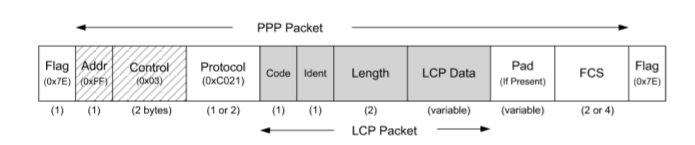
\includegraphics[width=500pt]{aufbau_ppp_frame}
  \end{center}
  \caption[Aufbau eines PPP-Frames]{Aufbau eines PPP-Frames \cite{tcpipillustrated}}
  \label{abb:aufbau_ppp_frame}
 \end{figure}

Diverse oben genannte Felder können in ihrer Länge variieren, da 
diese während des Verbindungsaufbaus vom \ac{LCP} ausgehandelt werden.

\paragraph{LCP Frame} Um die effizienteste Verbindungsart zu finden, benutzen PPP-Systeme
immer \ac{LCP}, welches korrekte Parameter aushandelt. LCP-Nachrichten in ausgetauschten
PPP-Frames enthalten somit alle Konfigurationsoptionen für die sich gerade aufbauende
Verbindung. Ist eine Konfiguration gefunden, die beide Knoten unterstützen folgt der
Link-Establishment-Prozess. Ist dieser erreicht müssen danach keine weiteren redundanten
Paketinformationen im Header mitgetragen werden.

Ein LCP-Frame ist wie folgt aufgebaut:
\begin{itemize}
	\item code (1 Byte) - hexadezimal - enhält den Messagetyp (als Codes spezifiziert)
	\item identifier (1 Byte) - hexadezimal - mit diesen werden Anfragen bzw. Antworten mit einzelnen LCP-Transaktionen in Verbindung gebracht
	\item length (2 Byte) - hexadezimal - beinhaltet die Länge der Nachricht (inklusive code, identifier, length, data)
	\item data (variabel) - hexadezimal - Nutzdaten
\end{itemize}

\ac{LCP} ist so entworfen, dass Hersteller ihre eigenen Optionen einsetzen können, ohne
selbige explizit über \ac{IANA} spezifizieren zu müssen. Dokumentiert ist dies in \textbf{RFC2153}.

\paragraph{Aufbauphasen} Nachfolgend werden die verschiedenen Aufbauphasen des
PPP-Protokolls erläutert. Im \Anhang{abb:aufbauphasen_pppverbindung} befindet
sich eine Abbildung, die diesen Vorgang illustriert.

%TODO: erst den Sinn der Phasen und dann wie das erzielt wird?
\textbf{Link Dead Phase:}
Quell- und Zielsystem fangen mit dieser Phase an und enden hiermit wieder.
Grundlage ist, dass außer (maximal) dem Link auf physischer Ebene,
keine Verbindung zwischen beiden Endpunkten besteht. Normalerweise
wird nach sicherstellen des physischen Links von einer Seite der
Aufbau der Verbindung initiiert. Dies geschieht meist mit einer Form von Modem.
Nach Abschluss der Initiierung beginnt die nachfolgende Phase.

\textbf{Link Establishment Phase:}
Das initiierende System sendet eine \ac{LCP}-Nachricht an das Zielsystem,
um Optionen anzufordern, die gesetzt werden sollen. Dazu gehören
Netzwerklayer-Protokoll, Authentifizierungsmethode und andere optionale
Funktionen. Sofern das Zielsystem alle angeforderten Optionen beherrscht,
kann dieses eine Bestätigung (\textbf{ACK}) an das Quellsystem senden.
Ist dies nicht der Fall, wird eine Anwort verfasst, die sowohl alle
\textit{nicht unterstützten} als auch alle \text{unterstützten} Optionen
enthält, damit das Quellsystem nach Empfang dieser Information eine
Verbindung initiieren kann, die in jedem Fall von beiden Seiten unterstützt
wird. Das erfolgreiche Abschließen dieser Phase führt zur nächsten Phase.

\textbf{Authentication Phase:}
Diese Phase ist optional. Ausgelöst wird sie durch das Vorhandensein einer
Authentifizierungsoption in der LCP-Konfigurationsnachricht.
Zur Auswahl stehen z.B. \ac{PAP} oder \ac{CHAP}.
Hierbei greift PAP auf Username und Passwort, CHAP auf einen komplexeren Informationsaustausch
mit einem Challenge-Response-Verfahren zurück. Der Erfolg führt immer zur nächsten
Phase führt, aber die Reaktion bei Misserfolg des Vorgangs ist protokollabhängig.

\textbf{Link Quality Monitoring:}
Diese Phase ist wie ihr Vorgänger ebenfalls optional - ebenfalls ausgelöst durch
die gewählt Option in der LCP-Nachricht.
Hier wird aus mehreren Protokollen gewählt. Eines davon ist standardisiert:
das 'Link Quality Report Protocol'. Registriert werden unter anderem der Linktraffic
sowie Fehlermeldungen.

\textbf{Network Layer Protocol Configuration:}
Wie bereits erwähnt unterstützt PPP  das multiplexen von Protokollen auf
Netzwerklayerebene. Für jedes einzelne, das eingesetzt wird,
führt das System einen separaten Prozess des Verbindungsaufbaus durch.
Jedes Netzwerklayerprotokoll verfügt über einen eigenes \ac{NCP} sowie \ac{IPCP}.
Vergleichbar ist dies mit dem Aufbau von \ac{LCP} - nur spezifischer.

\textbf{Link Open Phase:}
Nachdem alle individuellen Optionen und NCP-Exchanges erfolgreich durchgeführt wurden,
ist der Verbindungsaufbau komplett und Protokolldaten können jetzt über den aufgebauten
Link in beide Richtungen ausgetauscht werden.

\textbf{Link Termination Phase:}
Wird die Verbindung absichtlich (Ablauf der Session, Authentifizierungsfehler)
oder durch Fehler o.ä. getrennt, wird im Regelfall über \ac{LCP}
eine 'Terminate Request Message' versandt. Diese kann von der Gegenseite
angenommen (\textit{AKC}) werden, sofern die grundlegende Verbindung noch aktiv ist.
Beide Systeme sind dann wieder in der ursprünglich genannten 'Link Dead Phase'.
Eine Terminierung der Verbindung ist neben \ac{LCP} auch auf \ac{NCP}-Ebene möglich,
damit die PPP-Verbindung trotz 'Terminierung' bestehen bleibt.


\subsubsection{Architektur PPPoE}\label{subsubsection:architecture_pppoe}
Zur Realisierung der Verbindung zwischen Authentication Center und
Endgerät wurde in diesem Projekt aufgrund der Beschaffenheit des Raspberry Pis eine
Ethernetverbindung gewählt. Dieser wird das im vorangegangenen
Abschnitt erläuterte \ac{PPP}-Protokoll zugrunde gelegt.
In Ethernetframes werden PPP-Daten als Nutzdaten gekapselt.
Diese Methode wurde auch im realen Umfeld dazu entwickelt \acp{ISP} die
Möglichkeit zu geben Verbindungen über Kabelmodem oder DSL in Form
von Bridged-Topologien zu realisieren. Provider bewerkstelligen
so auch die Endpunktidentifikation, Accounting und Rechnungserstellung
(beschrieben wird der Standard in RFC2516).

\paragraph{Aufbauphasen}
Diese sind im Kontext einer PPPoE-Verbindung Discovery und Session.
Beide werden nachfolgend erläutert.

\paragraph{Discovery}
Der Client verwendet PPPoE-Frames in der Discovery-Phase dazu einen
Zugangspunkt zu finden.

Dies geschieht in den folgenden Schritten bzw. Frames:
\begin{enumerate}
\item PPPoE Active Discovery Initiation (PADI) - Ein Frame, vom Client
      gesendet an die Broadcastadresse 0xFF-FF-FF-FF-FF-FF.
      Falls vorhanden, werden weitere Parameter als Payload 
      mitgeschickt. (Codefeld:9; Session-ID:0)
\item PPPoE Active Discovery Offer (PADO) - Ein Frame, der von der
      Authentifizierungsstelle an die Unicast MAC-Adresse des
      initiierenden Client geschickt wird. Weitere Parameter wie
      Service-Name o.ä. können ebenfalls mitgeschickt
      werden. (Codefeld:7; Session-ID:0)
\item PPPoE Active Discovery Request (PADR) - Ein Frame, der vom Client
      an die Unicat MAC-Adresse der Authentifizierungsstelle geschickt
      wird. (Codefeld:25; Session-ID:0)
\item PPPoE Active Discovery Session-Confirmation (PADS) - Ein Frame,
      der von der Authentifizierungsstelle an die Unicast MAC-Adresse
      des Client geschickt wird. Er enthält alle ausgehandelten Daten
      mit der zugewiesenen Session-ID. (Codefeld:101; Session-ID:XX)
\item PPPoE Active Discovery Terminate (PADT) - Ein Frame,
      der von beiden Endpunkten geschickt werden kann. Er signalisiert
      die gewünschte Verbindungsterminierung des Absenders.
      (Codefeld:167)
\end{enumerate}

\paragraph{Session}
In der Sessionn-Phase, ist die PPPoE-Verbindung bereits erfolgreich
aufgebaut und Daten können ausgetauscht werden.
Dieser Zustand ist erreicht, sobald die Discovery-Phase
erfolgreich abgeschlossen ist.

\subsubsection{Roaring Penguin PPPoE}
Die eingesetzte Software zur Realisierung der PPPoE-Verbindung ist der
Roaring Penguin\footnote{\url{https://www.roaringpenguin.com/products/pppoe}} PPPoE-Server.

Er implementiert den PPPoE-Standard (\Verweis{subsubsection:architecture_pppoe}) auf Basis
von \textit{TCP/IP} und \textit{PPP} als eine \textit{Userland}-Anwendung.
Dementsprechend ist es nicht notwendig hierfür den Kernel zu patchen und neu zu bauen.
Ein einfaches installieren und konfigurieren genügt.

\paragraph{pppd}
Der im Userland installierte Dienst heißt pppd. Um eine Verbindung aufzubauen
erstellt er eine virtuelle Netzwerkschnittstelle (der Form ppp\textit{X}) und verknüpft diese
mit einem Pseudo-\ac{tty}. %TODO: Abkürzung? Was ist tty #CHECK
Typischerweise handelt es sich hier um einem seriellen Port \cite{roaringpenguinpres}).
Daten, die von diesem tty-Device empfangen werden, erscheinen durch das ppp\textit{X}-Device.

Logisch unterhalb des tty-Device wird dann über PPPoE mit einem ebenfalls durch den Server
asoziierten Ethernet-Interface kommuniziert (eth\textit{X}).

Der Informationsfluss findet somit in nachfolgender Hierarchie statt:
 \begin{figure}[htp]
  \begin{center}
   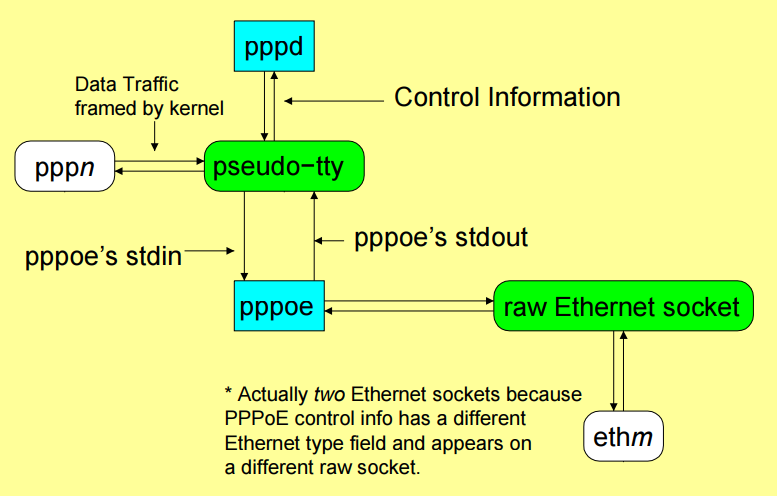
\includegraphics[width=300pt]{pppoe_roaringpenguin_2000}
  \end{center}
  \caption[Roaring Penguin PPPoE Devicehierarchie]{Roaring Penguin PPPoE Devicehierarchie \cite{roaringpenguinpres}}
  \label{fig:pppoe_roaringpenguin_devicehierarchy}
 \end{figure}

Ausgehend vom tty\textit{X}-Device kommen Daten in \ac{HDLC}-Frames zum Ethernet-Device.
Eingehende Pakete werden beim Ethernet-Device gerahmt und auf dem stdout an
das tty\textit{X}-Device weitergeleitet.

Kontroll- und Dateninformationen können bei Bedarf über unterschiedliche
Ethernet-Devices ausgetauscht werden.

\subsection{Ubuntu} % TODO: #edit vielleicht noch verschieben
\label{subsec:ubuntu}
Als Grundlage für die Umsetzung des Providers wird die Linuxdistribution Ubuntu\footnote{\url{http://www.ubuntu.com/}}
gewählt. In Desktop- sowie Serverumgebungen wird es zunehmend eingesetzt.
Unter anderem, da eines der Ziele des Projektes ist eine stabile
'Out-Of-The-Box'-Installation zu liefern. Neben der intuitiven Installation und dem
Betrieb wird auch jeweils eine \textit{LTS}-Version der aktuellen Veröffentlichung angeboten.
Hierbei steht das Akronym \textit{LTS} für Long Term Support und garantiert dem Anwender eine
Updateversorgung (an Paketen) über insgesamt fünf Jah-
re hinweg. Ebenso kann bei Bedarf separat technicher Support direkt von Canonical
Ltd. bezogen werden. Ubuntus initiale Veröffentlichung (Version 4.10) geht bis ins Jahr
2004 (20. Oktober) zurück und stammt von Debian GNU/Linux ab - es zeichnet sich
allerdings durch eine ebenso breite, allerdings darüber hinaus aktuellere Paketauswahl aus.

Motivation zum Einsatz von Ubuntu in der Version 14.04 LTS ist die bestehende Erfahrung
mit dieser Version in Verbindung mit dem PPPoE-Server von Roaring Penguin (Version 4.11).

\subsection{Raspberry Pi}

Die Hardwaregrundlage für das Endgerät bietet die Plattform eines Raspberry Pis, einem Kleincomputer.

\subsubsection{Raspberry Pi Foundation}
Entwickelt wird der Raspberry Pi von der Raspberry Pi Foundation\footnote{\url{https://www.raspberrypi.org}}
(registriert in Großbritannien). Ziel der Organisation ist es,
seit Veröffentlichung des ersten Modells, einen kostengünstigen
Computer vorrangig für Bildungszwecke zu entwerfen. Auf diesem
Weg soll sowohl Erwachsenen als auch Kindern der Zugang zum
Programmieren oder anderen wissenschaftlichen Anwendungsgebieten
erleichtert werden.

Bisher wurden seit der initialen Veröffentlichung im Februar 2012(\cite{rasppifoundweb})
drei Generationen in unterschiedlichen Ausführungen
entwickelt. Die Bezeichnung A(+) bzw. B(+) gibt jeweils Aufschluss
über die jeweilige Ausführung.

\subsubsection{Hardware Modell B}
Das in diesem Projekt eingesetzte Modell B der ersten Generation verfügt über folgende Hardwarekomponenten:
\begin{itemize}
\item CPU - 700 MHz Singlecore ARM1176JZF-S
\item RAM - 512 MB
\item Speicherslot - SDHC
\item Grafikprozessor - Broadcom VideoCore IV
\end{itemize}

\subsubsection{Betriebssystem}
Als Betriebssystem gibt es für den Raspberry Pi eine breite Auswahl.
Neben einer Vielzahl von Media-Center-Plattformen sind auch alle
Desktop- bzw. Server-Versionen gängiger Linux-Derivate verfügbar:
Arch Linux, Puppy Linux, Raspbian, openSUSE, Gentoo Linux, Ubuntu Mate,
CentOS, Slackware, ...

\paragraph{Raspbian}
Aufgrund hoher Stabilität und Verfügbarkeit aller benötigten Treiber
(u.a. dem SIM-Kartenleser) wurde die auf \textit{Debian GNU Linux}\footnote{\url{https://www.debian.org/}}
basierende Distribution \textit{Raspbian}\footnote{\url{https://www.raspbian.org/}} ausgewählt.
Es erbt somit alle Eigenschaftem vom übergeordneten Debianprojekt.
So auch den Paketmanager \textit{dpkg} mit ca. 35.000 vorkompilierten
Softwarepaketen - in einigen Fällen für den Betrieb mit dem
Raspberry Pi optimiert. Nicht vorpaketierte Software kann auf dem Raspberry
Pi durch vorhandensein einer Vielzahl von Libraries und Build-Tools
für die ARM-Architektur kompiliert werden.

Über den rein funktionalen Konsolenbetrieb hinaus, wird Raspbian standardmäßig mit den
Windowmanagern XFCE oder LXDE ausgeliefert.

Nachdem im Juni 2012(\cite{raspbianweb}) die erste
Version fertiggestellt wurde ist Raspbian nach wie vor aktiv
in Entwicklung. Momentan im stabilen Debian-Release \textit{Jessie}.
Selbiges wird auch zur Umsetzung des Endgerätes eingesetzt.
Die vorkompilierten Pakete stammen dementsprechend aus dem aktuellen
\textit{stable}-Zweig, der häufig vor allem im Umfeld des Serverbetriebes
anzutreffen ist. Die Ursache hierfür ist die Tatsache, dass das
Projekt Pakete erst nach einem langen Testprozess im \textit{unstable}-
sowie darauffolgenden \textit{testing-}Zweig für den \textit{stable}-Zweig
freigibt. Im Kontrast zu gängigen Desktop-Distributionen, die
im Vergleich zu Debian stärker auf Aktualität achten.

Neben den Zielen der Raspberry Pi Foundation verfolgt das Projekt
auch die Ziele des Debian/GNU-Projekts. Es ist dementsprechend unter
den \textit{Debian Free Software Guidelines}\footnote{\url{https://wiki.debian.org/DFSGLicenses}}
lizensiert und durch die Raspbian-Community unabhängig entwickelt.

%% PC/SC %%
\subsection{PC/SC}
%TODO: Die Kausalkette ist für mich nicht logisch #CHECK
Multitasking- und Multiuserbetrieb in modernen Betriebssystemen erfordert
auch das Bereitstellen eines Standards, um den Zugriff auf Chipkarten
mit mehreren (parallel arbeitenden) Teilnehmern zu organisieren. Ein Standard, der sich mit genau
dieser Problemstellung befasst ist der \textit{\ac{PC/SC}}-Standard.
Er abstrahiert die Kommunikation mit der Chipkarte so,
dass die Anwendung keine genaueren speziellen Informationen zur verwendeten
Karte benötigt. Lediglich die Kommunikation mit dem Standard
konformen Lesegerät muss durch den Treiber sichergestellt werden.

% \subsubsection{Die PC/SC-Workgroup}
Entwickelt wurde PC/SC von verschiedenen Herstellern. Hauptsächlich
Gemalto, Microsoft, Infineon und Toshiba.

\subsubsection{Spezifikation und Aufbau der Schnittstelle}
Die Spezifikation definiert Schnittstellen, die den Zugriff auf Chipkarten ausgehend
von mehreren Applikationen beziehungsweise Nutzern ermöglichen. Grundlegend
dafür benötigt werden neben dem Standardkonformen Treiber ein \ac{IFD} und
eine \textit{PC/SC}-konforme Chipkarte (\ac{ICC} nach ISO7816-1,2 und 3).

 \begin{figure}[htp]
  \begin{center}
   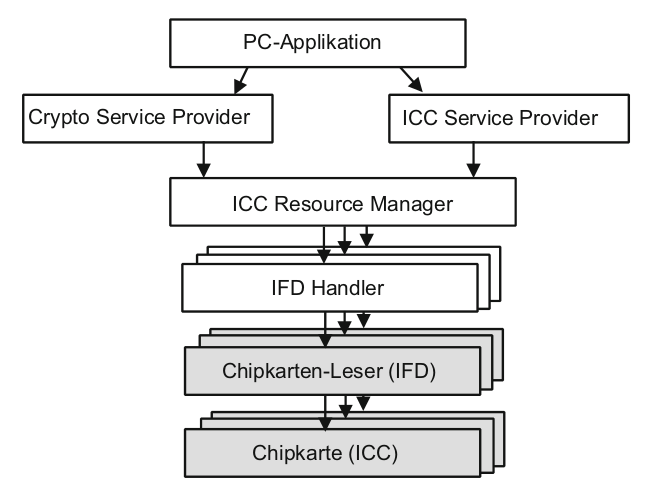
\includegraphics[width=300pt]{pcscspec_chipkartenitsicherheit}
  \end{center}
  \caption[Architektur des PC/SC-Standards]{Architektur des PC/SC-Standards \cite{spitz11}}
  \label{abb:architektur_pcsc}
 \end{figure}

Der Unterschied zum ähnlichen CT-API-Standard fängt in der Ebene
des \textit{ICC Resource Managers} an. Also der Abstraktion der
APDU-Schnittstelle in der Chipkartenmiddleware \cite{spitz11}.
Selbiger Manager organisiert sowohl die Vergabe von Terminals inklusive
der vorhandenen Chipkarte, als auch das Zuordnen zusammenhängender
APDU-Kommandoketten.

Losgelöst davon können Daten auf der Chipkarte abgelegt werden. Im Umfeld
der SIM-Karte sind dies Kontakte, SMS, o.ä. Hierfür zuständig ist der
\textit{ICC Service Provider}. Ebenfalls dazu gehören administrative Dateisystemzugriffe
wie das Ändern des PIN-Codes.

Der \textit{Cryptographic Service Provider} ist die ausführende Komponente
der auf der Chipkarte implementierten Algorithmen zur Authentifizierung mittels
Kryptoalgorithmen. Auslöser für die Aufteilung in zwei Schnittstellen -
\textit{Crypto Service Provider} und \textit{ICC Service Provider} sind
rechtliche Grundlagen. In manchen Staaten ist der Import von
Verschlüsselungtechnologien auf diesem Weg untersagt.

Unter Einhaltung des Standards ist es mit oben genannter Architektur möglich,
dass parallel aus verschiedenen Anwendungen auf unterschiedliche Konstellationen
von Chipkarten und Lesern zugegriffen wird.

Sowohl unter Windows als auch in vielen Linux-Distributionen sind
\textit{PC/SC-Treiber} mittlerweile verbreitet.

\subsubsection{PCSClite}
Die unter Linux-Distributionen verfügbare Version ist
PCSClite\footnote{\url{https://pcsclite.alioth.debian.org/}}.
Das von David Corcoran gestartete Projekt M.U.S.C.L.E
(Movement for the Use of Smart Cards in a Linux Environment)
wird mittlerweile hauptsächlich von Ludovic Rousseau
weitergeführt\cite{pcscliteweb}.

Neben diversen Linux-Distributionen werden auch Mac OSX und diverse
BSD- sowie Unix-Derivate unterstützt.

\subsection{Die Sprache Python}
\subsubsection{Grundlagen}
\textit{Python} ist eine seit 1991 frei veröffentlichte Programmiersprache. Sie zählt
zu den interpretierten Programmiersprachen. Primäre Ziele der Sprache sind zusammengefasst:
\begin{itemize}
\item Lesbarkeit
\item Kompaktheit
\end{itemize}
Somit wird neben etablierten Sprachen eine Alternative für sowohl umfangreiche Softwareprojekte
als auch kleinere Einsatzgebiete wie Skripting im Heimcomputerbereich angeboten.

\textit{Python} konzentriert sich nicht ausschließlich auf ein einziges Programmierparadigma.
Es unterstützt objektorientierte, funktionale sowie prozedurale Programmierung. Zusätzliche
Paradigmen (unter anderem auch logische) können über Erweiterungen nachgerüstet werden.
Weiterhin verfügt \textit{Python} dynamische Typisierung und automatisches Speichermanagement. Aus
diesen Gründen ist \textit{Python} vor allem auch für Einsteiger in das Thema der Programmierung
gut geeignet. Nichts desto Trotz ist \textit{Python} auch aufgrund seiner hohen Flexibilität
bei erfahrenen Entwicklern verbreitet.

In vielen Linux-Distributionen gehört \textit{Python} im gewissem Umfang zur Standardinstallation.
Mit dem ausgelieferten Interpreter können plattformübergreifend Programme ausgeführt werden. Bei
Bedarf ist es möglich auf eine Große Anzahl von Paketen in Standardbibliotheken zuzugreifen.

In seltenen Fällen kann es auch notwendig sein Binärcode auszuliefern, ohne den
\textit{Python}-Interpreter zu installieren. Hierfür existieren Tools von Drittanbietern,
die aus vorliegendem \textit{Python}-Code ausführbare Programme generieren. Ein Beispiel hierfür
ist \textit{py2exe}\footnote{\url{http://www.py2exe.org/}}.

\subsubsection{Motivation zur Nutzung}
Die Entscheidung für diese Programmiersprache fällt vor allem aus dem Grund, dass bereits eine
Vielzahl von Skripten aus kleineren Projekten im Bereich der Kommunikation mit \textit{SIM}-Karten
(also auf der Seite der \ac{MS}) existieren. An diese Skripte kann angeschlossen werden. Nachfolgend werden die zugrunde liegende
Skripte näher erläutert. Diese werden für die Umsetzung dieser Studienarbeit verwendet sowie
in ihrer Funktion erweitert.

\subsection{pysim} % TODO #edit bei bedarf noch syntax etc nachtragen
Pysim\footnote{\url{https://github.com/kevinprince/pysim}} ist ein
python-Skript, geschrieben von Kevin Prince,
welches Operationen direkt auf der SIM-Karte implementiert.
Sowohl Kryptoalgorithmen wie Milenage als auch administrative Dateisystemzugriffe
bis hin zur Verwaltung von Telefonbuch, SMS oder ähnlichem.
Unterstützt wird der GSM-Authentifizierungsvorgang.

Pysim kennt verschiedene Modi und nimmt dementsprechend unterschiedliche
Parameter entgegen. Verfügbare Parameter sind Chipkartentyp, verwendetes
Device (im Betriebssystem /dev/ttyX) und Baudrate\cite{pysimprince}.

Über den normalen Betrieb einer SIM-Karte (also Authentifizierung, Auslesen, etc.)
ist es mit Pysim auch möglich Werte auf programmierbaren SIM-Karten zu setzen.

Neben abgeschlossenen Skripten ist auch die interaktive Nutzung auf der
python-Shell verwendbar.

\subsection{osmo-sim-auth}
\label{subsec:osmosim}
\textit{Osmo-sim-auth}\footnote{\url{http://openbsc.osmocom.org/trac/wiki/osmo-sim-auth}}
überschneidet sich im Unfang angebotener Funktionen mit \textit{pysim}. Hauptsächlich ist es,
genau wie \textit{pysim} eine Implementierung in python, um den Authentifizierungsprozess
einer Chipkarte zu steuern. Es basiert ebenfalls auf der Grundlage des
\textit{PCSClite}-Treibers und der \textit{pyscard}-Library.

Ein Unterschied zwischen beiden python-Skripten stellte sich bei der
Realisierung der Kommunikation in der Praxis heraus:
Während \textit{pysim} auch die Programmierung von Chipkarten anbietet, ist
\textit{osmo-sim-auth} dazu in der Lage über \ac{GSM}- hinaus auch
eine \ac{UMTS}-Authentifizierung zu leiten.
Der jeweilige Modus wird über Parameter übermittelt.
Dementsprechend verfügt \textit{osmo-sim-auth} auch über die Funktion der
Resynchronisation bezüglich der \ac{SQN}-Nummer\cite{osmosimweb}.

Entwickelt wird es vom Osmocom OpenBSC-Project, welches sich damit
beschäftigt eine (A)GPL-lizenzierte Implementierung für den
GSM/3GPP-Protokollstack zu erzielen. Neben der Authentifizierung
in direkter Kommunikation mit der SIM-Karte werden auch folgende
Funktionalitäten durch das Projekt realisiert:
\ac{BSC},\ac{MSC},\ac{HLR},\ac{AuC},\ac{VLR}, und \ac{EIR}\cite{osmocombscweb}.

\subsection{pyscard}
Zur Verwendung des Tools \textit{pysim} oder \textit{osmo-sim-auth} wird eine python-Bibliothek benötigt,
die Smartcard-Support für Python bereitstellt. Diese Bibliothek
ist pysim. Sie fungiert als Schnittstelle zwischen dem Treiber \textit{PC/SC}
beziehungsweise \textit{PCSClite} und der Python-Anwendung 
(dargestellt im \Anhang{abb:pyscard_schema}).

Implementierte Funktionen sind das Prüfen der gesteckten bzw. nicht gesteckten
Chipkarte, der darauffolgende Verbindungsaufbau sowie das Versenden und
Empfangen von APDUs in hexadezimaler Darstellung.
Nach erfolgreichem Verbindungsaufbau kann somit eine Kommunikation via
APDUs stattfinden.

Veröffentlicht wurde pyscard als freie Software unter der
\textit{GNU Lesser General Public License}.

%% Programmiersprache C %%
\subsection{Die Sprache C}
 C ist eine prozedurale Programmiersprache, die nicht für einen speziellen
 Anwendungsfall entwickelt wurde. Sie hat einen hohen Verbreitungsgrad
 und ist laut \ac{IEEE} Spectrum\footnote{\url{http://spectrum.ieee.org/computing/software/the-2015-top-ten-programming-languages} [besucht am 17.05.16]}
 und RedMonk\footnote{\url{http://redmonk.com/sogrady/2016/02/19/language-rankings-1-16/} [besucht am 17.05.16]}
 unter den 10 beliebtesten Programmier\-sprachen. C ist eine sehr hardware\-
 nahe Sprache und wird deshalb oft als Ersatz für Assembler eingesetzt. In
 diesem Kapitel soll kurz auf die Geschichte eingegangen werden, was es
 bedeutet, dass die Sprache prozedural ist und welche Besonderheiten C
 aufweist.

 \subsubsection{Geschichte}
  Die Entwicklung von C hängt stark zusammen mit der Entwicklung des Unix-Systems.
  Dieses wurde ursprünglich in Assembler geschrieben und nun wurde
  überlegt den Code neu zu schreiben, allerdings in B. Mit B ließen sich jedoch
  einige der Unix-Features nicht umzusetzen, wie beispielsweise die Byte-Adressierung.
  
  Deshalb wurde 1972 C von Dennies Ritchie bei Bell Labs entwickelt. Die Portabilität war
  dabei zu Beginn nicht beabsichtigt, stattdessen war C nur für Unix-Systeme entwickelt
  worden. Allerdings wurden schnell Compiler auch auf andere Systeme portiert. 1973
  war C dann leistungsfähig genug, dass der Großteil des Unix Kernels in C geschrieben war.
  
  C wurde Ende der 70er auf verschiedenen Rechensystemen, wie Mainframecomputer und
  Heimrechnern von implementiert. Dies bewegte vermutlich das American National Standards
  Institude dazu, 1983 eine Komitee zu gründen, was sich um eine Standardspezifikation von
  C kümmert. Das Komitee, X3J11, veröffentlichte 1989 seinen ersten Standard, der oft auch
  als ANSI C, Standard C oder C89 bekannt ist.
  
  Nach der Weitergabe des Standards an die \ac{ISO} 1990 wurde dieser weiterentwickelt und
  führte zu zwei weiteren Standards in 1999 (C99) und 2011 (C11). Unterstützt wird von den
  Compilern C89 und oft auch C99, wohingegen C11 nicht sehr verbreitet ist. \nocite{ritchie93}
 
 \subsubsection{Prozedurales Konzept}
  

 \subsubsection{Besonderheiten}
 

\subsection{Projektumsetzung}
 \subsubsection{Anforderungen}
 Zu Beginn, und teilweise auch während des Projektes, wurden Anforderungen
 an das Projekt gestellt, die umgesetzt werden sollen und Grenzen gesetzt, die
 dem Projekt einen Rahmen vorgeben. Außerdem wurden Meilensteine definiert,
 um der Projektumsetzung mehr Struktur zu geben.
 
 In Kapitel \Verweis{idee-arbeit} wurde bereits angesprochen, dass hardwareseitig
 ein Raspberry Pi mit einem Kartenleser als \ac{UE} dienen soll und der Netzprovider
 simuliert wird auf einer virtuellen Maschine. Die Kommunikation der beiden Geräte
 wird über eine \ac{PPPoE}-Verbindung realisiert. Was nicht simuliert wird, ist der
 \ac{SGSN}, da dafür eine weitere virtuelle Maschine aufgesetzt werden muss und die
 Funktionalität des Knotens darauf reduziert wäre RES und XRES (vgl. Kapitel \ref{authentifizierungsvorgang})
 miteinander zu vergleichen.
 
 Der Vergleich der beiden Werte RES und XRES wird allerdings auch nicht an anderer
 Stelle umgesetzt, sondern fällt weg, ebenso wie bei der Resnchronisation der Vergleich
 von MAC-S mit XMAC-S. Beide Vergleiche werden gemacht um sicher zu stellen, dass
 der jeweils andere Kommunikationspartner nicht korrupt ist. Da in diesem Projekt eine
 PPPoE-Verbindung genutzt wird, ist sichergestellt, dass beide Partner nicht korrupt sind
 und eine Überprüfung deshalb überflüssig.
 
 Da das Kernziel eine erfolgreiche Authentifizierung ist, werden die nötigen Funktionen
 für sowohl die Synchronisation, als auch die Resynchronisation umgesetzt. Die Datenbank
 in der der aktuelle SQN, beziehungsweise SEQ, gespeichert werden fällt jedoch weg, da
 diese bei nur einer USIM wieder zusätzlicher Aufwand bedeutet. \\
 Da es außerdem nur um die Authentifizierung geht, aber nicht die Kommunikation zwischen
 beiden Seiten, wird vom simulierten AuC kein CK oder IK generiert. \\
 Damit bleibt, dass bis auf \emph{f3} und \emph{f4}, alle Funktionen, die in Kapitel \Verweis{milenage}
 genannt wurden, korrekt umgesetzt werden sollen.
 
 Zur korrekten Umsetzung der Milenage-Funktionen gehört ebenfalls eine Eigen\-implementierung
 des AES-Algorithmus, aber nur für eine Blocklänge von 128 Bits, da der Milenage-Algorithmus
 keine anderen Blocklängen benötigt.
 
 Bei beiden Algorithmen geht es zudem nicht um Geschwindigkeit oder Ressourcenverbrauch.
 Das soll heißen, dass bei der Implementierung dieser nicht daraufhin optimiert wird, dass wenig
 Speicherplatz benötigt wird oder das Programm besonders schnell ist. Stattdessen ist lediglich
 wichtig, dass beide Algorithmen korrekt implementiert werden und am Ende die Werte generieren
 die für die Eingabeparameter zu erwarten sind.
 
 \paragraph{Meilensteine} Die Meilensteine, die für das Projekt definiert wurden lauten wie folgt:
 \begin{description}
 \item [27.10.2015] Die Grundlagen für die Authentifizierungs\-algorithmen sollen bekannt und verstanden sein
 \item [07.12.2015] Das Auslesen einer USIM soll funktionieren, alternativ soll eine USIM emuliert werden können
 \item [01.02.2016] Der virtuelle Netzbetreiber soll gemäß der Spezifikationen funktionieren, für die nötigen Funktionen
 \item [29.02.2016] Die USIM soll in den Authentifizierungsprozess eingebunden werden, also mit dem virtuellen Netzbetreiber kommunizieren
 \item [17.04.2016] Die Studienarbeit ist bis zu diesem Zeitpunkt fertig geschrieben
 \item [30.05.2016] Die Studienarbeit muss abgegeben werden
 \end{description}
 
 Durch die Meilensteine ist eine klare Struktur gegeben und es gibt einen Zeitpuffer am Ende,
 um eventuell auftretende Komplikationen und Verzögerungen ausgleichen zu können ohne den
 Erfolg des Projektes zu gefährden.

 \subsubsection{Unterstützende Tools}
  Im Projekt werden einige Tools genutzt, die die Arbeit unterstützen und die Kommunikation
  unter den beiden Autoren vereinfacht. Trello und Git(hub) sollen hier kurz vorgestellt werden,
  da sie eine große Hilfe waren.

  \paragraph{Trello}
  Die web-basierte Projekt\-management\-software Trello wird vom US-amerikanischen Unternehmen
  ``Fog Creek Software'' betrieben. Gegründet wurde es am 13. September 2011 und erfreut sich  in
  letzter Zeit immer mehr Beliebtheit, sodass es seit Mitte 2015 auch auf Deutsch existiert. \\
  Wenn man bei Trello angemeldet ist, kann man mehreren sogenannten Boards zugeordnet sein. In
  diesen Boards gibt es dann Listen. So kann mit Trello schnell ein Scrum- oder Kanban-Board
  erstellt werden. Man ist darauf jedoch nicht festgelegt, weshalb die Software ziemlich
  nutzungsoffen ist. In den Listen lassen sich dann Karten anlegen, welche sowohl Text, als auch
  Bilder und Checklisten enthalten können.

  \paragraph{Git}
  Um den Programmcode und das Schreiben dieser Arbeit zu vereinfachen, wurde Git genutzt. Dies ist
  eine quelloffene verteilte Versionierungsverwaltung, die vom Linux Gründer Linus Torvalds entwickelt
  wurde. Der Grund dafür war, dass die Entwickler des Linuxkernels lange BitKeeper genutzt haben
  für die Versonsverwaltung, aber dies konnte durch eine Lizenzänderung nicht mehr genutzt werden,
  weshalb Torvalds sich entschied seine eigene Verwaltung zu bauen, die seine Anforderungen erfüllt. \\
  Im Gegensatz zu beispielsweise Subversion, gibt es nicht einen zentralen Server, auf dem die komplette
  Historie gespeichert ist, sondern jeder Client ist auch ein Server und hält die Historie bereit. Dies
  ermöglicht dem Nutzer einige Interaktionen durchzuführen ohne an das Internet angebunden zu sein. \\
  Git hat bewiesen, dass es stabil ist, da viele größere Projekte wie Android oder Eclipse damit ihre
  Projekte entwickeln.